\documentclass[11pt, oneside]{article}   	% use "amsart" instead of "article" for AMSLaTeX format
\usepackage{geometry}                		% See geometry.pdf to learn the layout options. There are lots.
\geometry{a4paper}                   		% ... or a4paper or a5paper or ... 
%\geometry{landscape}                		% Activate for for rotated page geometry
%\usepackage[parfill]{parskip}    		% Activate to begin paragraphs with an empty line rather than an indent
\usepackage{graphicx}				% Use pdf, png, jpg, or eps§ with pdflatex; use eps in DVI mode
\usepackage{array}							% TeX will automatically convert eps --> pdf in pdflatex		
\usepackage{amssymb}
\usepackage{cite}
\usepackage[final]{fixme}
\usepackage{pdfpages}
\usepackage{tabularx}
\usepackage{fancyheadings}
\usepackage{lastpage}

\parskip 6pt % 1pt = 0.351 mm
\parindent 0pt

%\title{Requirement Engineering Process in AMIDST}
%\author{The handsome AMIDST guys et. al.}
%\date{Latest version, \today}							% Activate to display a given date or no date

\pagestyle{fancy}
\lhead{\tiny FP7-ICT 619209 / AMIDST}
\chead{\tiny Page {\thepage} of \pageref{LastPage} \\}
\rhead{\tiny Public}
\renewcommand{\footrulewidth}{0.4pt}
\cfoot{}




\begin{document}

%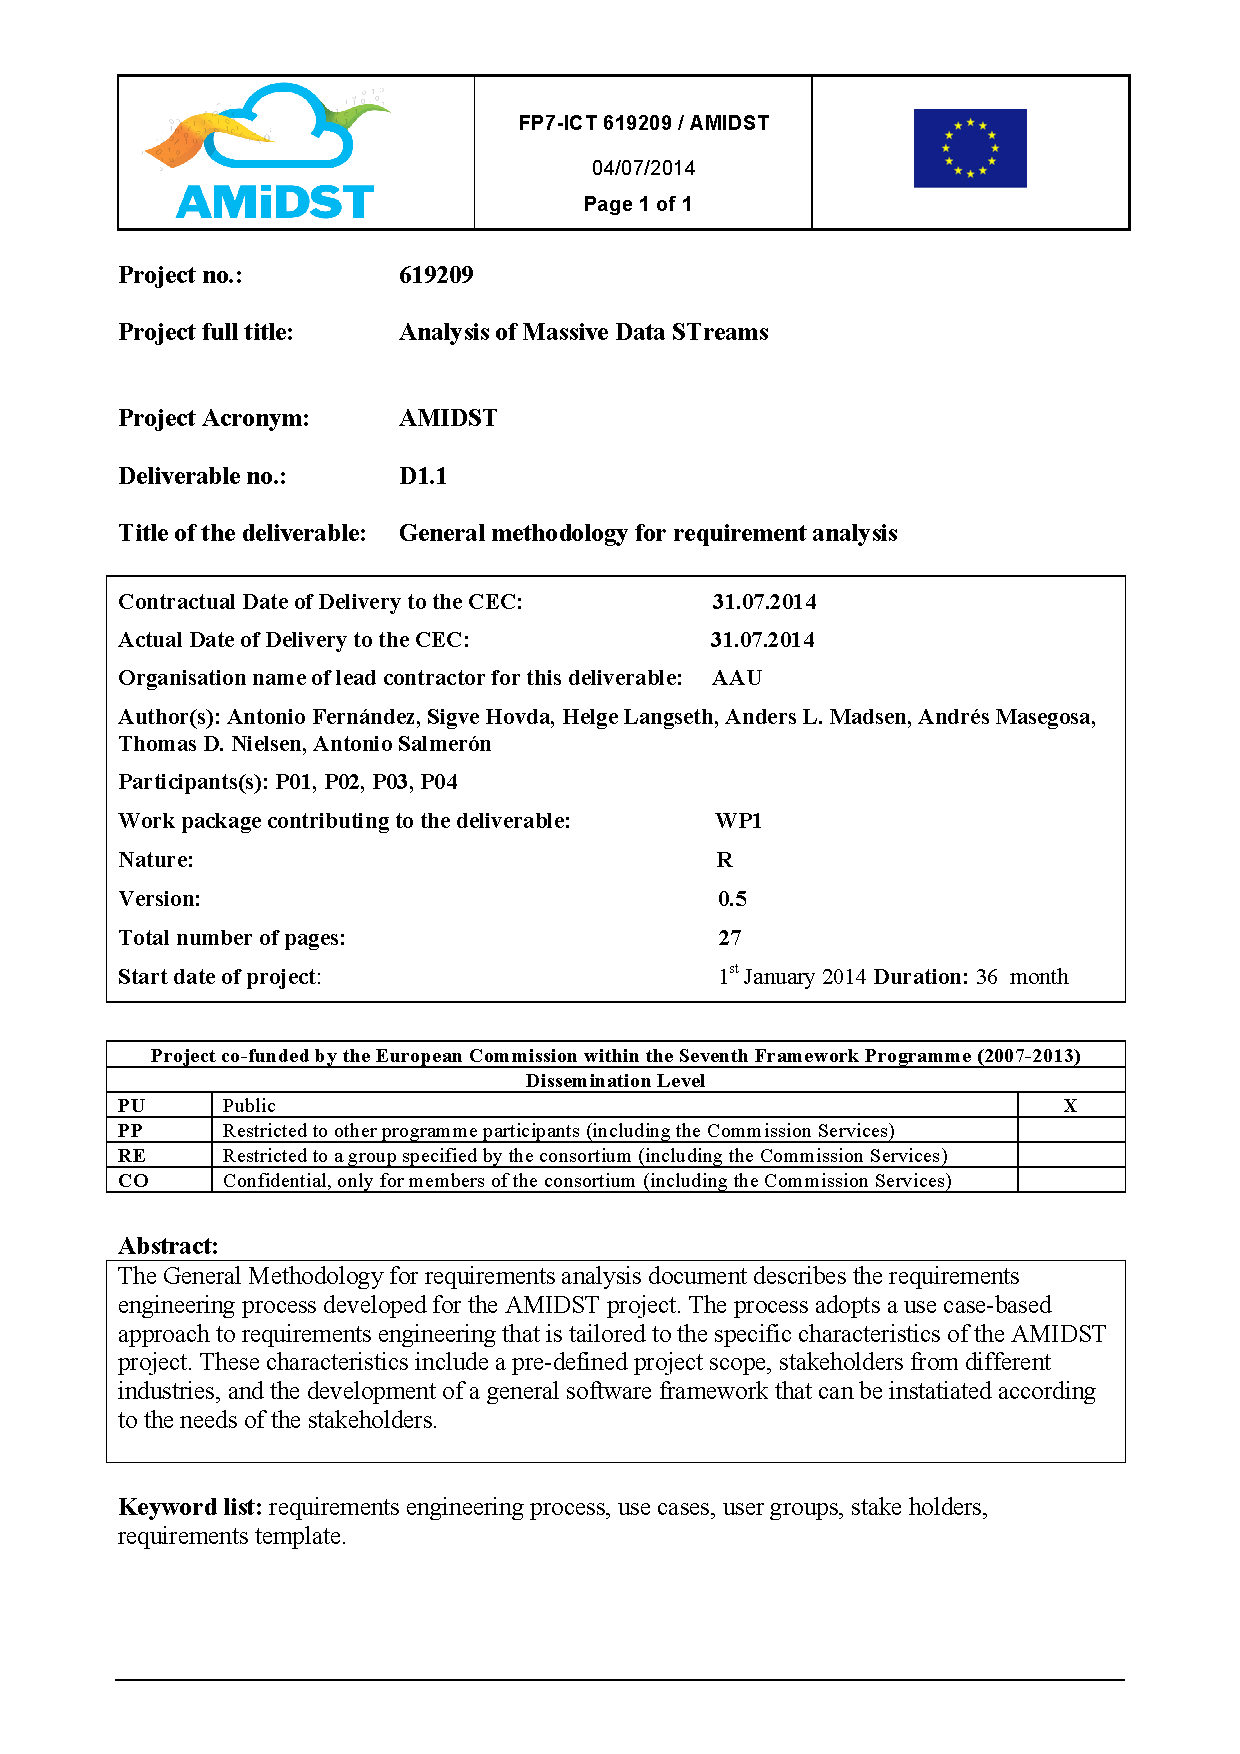
\includepdf{AMiDST_Template_Deliverables.pdf}

%\maketitle
%
%\begin{abstract}
%\end{abstract}
%



% Table of contents
\tableofcontents

\newpage

% Document History

\section*{Document history}

\begin{table}[htbp]
  \centering
  \begin{tabularx}{\linewidth}{|p{17mm}|p{17mm}|X|X|}\hline
    {\bf Version} & {\bf Date} & {\bf Author (Unit)} & {\bf Description} \\ \hline \hline
    v0.3 &  &  & First draft finished  \\ 
\hline
  \end{tabularx}
\end{table}

\newpage


% Document History

\section{Executive summary}

\newpage


%%%%%%%%%%%%%%%%%%%%%%%%%%%%%%%%%%%%%%%%%
\newpage
\section{Use Case - Data bases (DB)}
\label{UseCase:DB}

\begin{description}
\item[Priority:] Must
\item[Deadline:] M15
\item[Responsible:] Sigve
\end{description}

\subsubsection*{Description of the use case}

This use case will cover the managing of the data bases that will be used by the models and learning algorithms implemented in the toolbox.  

\subsubsection*{Must-Requirements list of the use case}

\begin{enumerate}
\item Data on memory
\item Data on disk
\end{enumerate}

\subsubsection*{Should-Requirements list of the use case}

\begin{enumerate}
\item Data on stream
\end{enumerate}

\subsubsection*{Could-Requirements list of the use case}

\begin{enumerate}
\item Short Description
\end{enumerate}



\subsection{Data On Memory}
\label{Functionality:ID}

\begin{description}
\item[Priority:] Must/Should/Could
\item[Deadline:] M?
\item[Responsible:]
\item[Code-Package:]
\end{description}

\subsubsection*{Description}

Enter a textual description of the functionality. Link to other functionalities if needed. 


\subsubsection*{Must-Requirements List}

\begin{itemize}
\item \textbf{Requirement-ID:} Short Description
\end{itemize}

\subsubsection*{Should-Requirements List}

\begin{itemize}
\item \textbf{Requirement-ID:} Short Description
\end{itemize}

\subsubsection*{Could-Requirements List}

\begin{itemize}
\item \textbf{Requirement-ID:} Short Description
\end{itemize}


\subsection{Data On Disk}
\label{Functionality:ID}

\begin{description}
\item[Priority:] Must/Should/Could
\item[Deadline:] M?
\item[Responsible:]
\item[Code-Package:]
\end{description}

\subsubsection*{Description}

Enter a textual description of the functionality. Link to other functionalities if needed. 


\subsubsection*{Must-Requirements List}

\begin{itemize}
\item \textbf{Requirement-ID:} Short Description
\end{itemize}

\subsubsection*{Should-Requirements List}

\begin{itemize}
\item \textbf{Requirement-ID:} Short Description
\end{itemize}

\subsubsection*{Could-Requirements List}

\begin{itemize}
\item \textbf{Requirement-ID:} Short Description
\end{itemize}


\subsection{Data On Stream}
\label{Functionality:ID}

\begin{description}
\item[Priority:] Must/Should/Could
\item[Deadline:] M?
\item[Responsible:]
\item[Code-Package:]
\end{description}

\subsubsection*{Description}

Enter a textual description of the functionality. Link to other functionalities if needed. 


\subsubsection*{Must-Requirements List}

\begin{itemize}
\item \textbf{Requirement-ID:} Short Description
\end{itemize}

\subsubsection*{Should-Requirements List}

\begin{itemize}
\item \textbf{Requirement-ID:} Short Description
\end{itemize}

\subsubsection*{Could-Requirements List}

\begin{itemize}
\item \textbf{Requirement-ID:} Short Description
\end{itemize}



%%%%%%%%%%%%%%%%%%%%%%%%%%%%%%%%%%%%%%%%%

\newpage
\section{Use Case - Basic Data Structures (BS)}
\label{UseCase:BS}

\begin{description}
\item[Priority:] Must
\item[Deadline:] M15
\item[Responsible:] 
\end{description}

\subsubsection*{Description of the Use Case}

This use case will cover the basic data structures to handle the probabilistic graphical models belonging to the AMIDST model class, and to be included in the toolbox (a tentative list is given below).

On the other hand, information about possible models to be plug-in into the toolbox beyond the project is also desirable to be indicated.  

\subsubsection*{Must-Requirements List of the Use Case}

\begin{enumerate}
\item Static Bayesian network (BN)
\item Two-time slice dynamic Bayesian network (2T-DBN)
\item Bounded dynamic Bayesian network 
\end{enumerate}

\subsubsection*{Should-Requirements List of the Use Case}

\begin{enumerate}
\item Additional operations for learning Bayesian networksS
\end{enumerate}

\subsubsection*{Could-Requirements List of the Use Case}

\begin{enumerate}
\item Factor graphs
\end{enumerate}
\subsection{Variable}
\label{Functionality:ID}

\begin{description}
\item[Priority:] Must/Should/Could
\item[Deadline:] M?
\item[Responsible:]
\item[Code-Package:]
\end{description}

\subsubsection*{Description}

Enter a textual description of the functionality. Link to other functionalities if needed. 


\subsubsection*{Must-Requirements List}

\begin{itemize}
\item \textbf{Requirement-ID:} Short Description
\end{itemize}

\subsubsection*{Should-Requirements List}

\begin{itemize}
\item \textbf{Requirement-ID:} Short Description
\end{itemize}

\subsubsection*{Could-Requirements List}

\begin{itemize}
\item \textbf{Requirement-ID:} Short Description
\end{itemize}


\subsection{Static Model Header}
\label{Functionality:ID}

\begin{description}
\item[Priority:] Must/Should/Could
\item[Deadline:] M?
\item[Responsible:]
\item[Code-Package:]
\end{description}

\subsubsection*{Description}

Enter a textual description of the functionality. Link to other functionalities if needed. 


\subsubsection*{Must-Requirements List}

\begin{itemize}
\item \textbf{Requirement-ID:} Short Description
\end{itemize}

\subsubsection*{Should-Requirements List}

\begin{itemize}
\item \textbf{Requirement-ID:} Short Description
\end{itemize}

\subsubsection*{Could-Requirements List}

\begin{itemize}
\item \textbf{Requirement-ID:} Short Description
\end{itemize}


\subsection{Dynamic Model Header}
\label{Functionality:ID}

\begin{description}
\item[Priority:] Must/Should/Could
\item[Deadline:] M?
\item[Responsible:]
\item[Code-Package:]
\end{description}

\subsubsection*{Description}

Enter a textual description of the functionality. Link to other functionalities if needed. 


\subsubsection*{Must-Requirements List}

\begin{itemize}
\item \textbf{Requirement-ID:} Short Description
\end{itemize}

\subsubsection*{Should-Requirements List}

\begin{itemize}
\item \textbf{Requirement-ID:} Short Description
\end{itemize}

\subsubsection*{Could-Requirements List}

\begin{itemize}
\item \textbf{Requirement-ID:} Short Description
\end{itemize}


\subsection{Directed acyclic graph (DAG)}
\label{DAG:ID}

\begin{description}
\item[Deadline:] M12
\item[Responsible:]
\item[Code-Package:] \texttt{eu.amidst.core.models}
\end{description}


\subsubsection*{Description}

The class Directed acyclic graph (DAG) defines the Bayesian network graphical structure over a list of static variables.

\subsubsection*{Detailed functionality}

\begin{itemize}
\item It defines the parent set for each variable.
\item It test and detect if a DAG contains cycles or not.
\end{itemize}
\newpage
\subsection{Distributions}
\label{Distributions:D}

\begin{description}
\item[Deadline:] M15
\item[Responsible:] Antonio Fern\'andez
\item[Code-Package:] \texttt{eu.amidst.core.distributions}
\end{description}

%--------------------------------------------------------------------------------------------
\subsubsection*{Description}
%--------------------------------------------------------------------------------------------

This functionality addresses the set of conditional probability distributions considered to be included in the toolbox. Variables with Gaussian and multinomial distributions are modeled. The variables arrangement in the model structure gives rise to the different types of probability distributions, one for each variable in the network. 

This functionality is tightly connected to functionality \texttt{Variable} and \texttt{DAG} to know both the type and the set of parents of each variable.

%--------------------------------------------------------------------------------------------
\subsubsection*{Detailed functionality}
%--------------------------------------------------------------------------------------------

The type and the set of parents of each variable determine the different defined probability distributions as follows:

\begin{itemize}
\item Multinomial variable with no parents
\item Multinomial variable with multinomial parents.
\item Gaussian variable with no parents.
\item Gaussian variable with multinomial parents.
\item Gaussian variable with Gaussian parents. 
\item Gaussian variable with a mixture of multinomial and Gaussian parents. 
\end{itemize}

Note that a multinomial variable is not allowed to have Gaussian parents and therefore it has not been included in the list above.

Multinomial parents are only used for indexing the set of possible distributions of the variable, so the functionality when no multinomial parents reduces to the general case.


%--------------------------------------------------------------------------------------------
\subsubsection*{Code example}
%--------------------------------------------------------------------------------------------

This is brief code fragment showing the definition of the distribution for a variable \texttt{var} given the set of its parents:

\begin{table}[H]
\begin{tabular}{l} \hline

        \texttt{ParentSet parentSet = this.getDAG().getParentSet(var);}\\
        \texttt{int varID = var.getVarID();}\\

        \texttt{this.distributions[varID]= }\\
         \texttt{~~~~~DistributionBuilder.newDistribution(var, parentSet.getParents());}\\
        \texttt{parentSet.blockParents();}\\ \hline 

\end{tabular}
\end{table}


            

            
            
           
\subsection{Bayesian network}
\label{BNs:ID}

\begin{description}
\item[Deadline:] M12
\item[Responsible:] 
\item[Code-Package:] \texttt{eu.amidst.core.models}
\end{description}

\subsubsection*{Description}

This class defines a static Bayesian network using the already specified graphical structure (DAG) along with the conditional probability distribution of each variable given the set of its parents.  

\subsubsection*{Detailed functionality}

\begin{itemize}

\item The distribution of each variable in the Bayesian network is initialised and specified according to its type and the type of its potentiel parent set. 

\item After this step, the set of parents of each variable becomes unmodifiable.

\end{itemize}
\subsection{2TDBN}
\label{Functionality:ID}

\begin{description}
\item[Priority:] Must/Should/Could
\item[Deadline:] M?
\item[Responsible:]
\item[Code-Package:]
\end{description}

\subsubsection*{Description}

Enter a textual description of the functionality. Link to other functionalities if needed. 


\subsubsection*{Must-Requirements List}

\begin{itemize}
\item \textbf{Requirement-ID:} Short Description
\end{itemize}

\subsubsection*{Should-Requirements List}

\begin{itemize}
\item \textbf{Requirement-ID:} Short Description
\end{itemize}

\subsubsection*{Could-Requirements List}

\begin{itemize}
\item \textbf{Requirement-ID:} Short Description
\end{itemize}



%%%%%%%%%%%%%%%%%%%%%%%%%%%%%%%%%%%%%%%%%



%%%%%%%%%%%%%%%%%%%%%%%%%%%%%%%%%%%%%%%%%

\bibliographystyle{splncs}
%\bibliography{re}

%\appendix
%\section{Formal framework for requirements elicitation}
%\label{sec:form-fram-requ}
%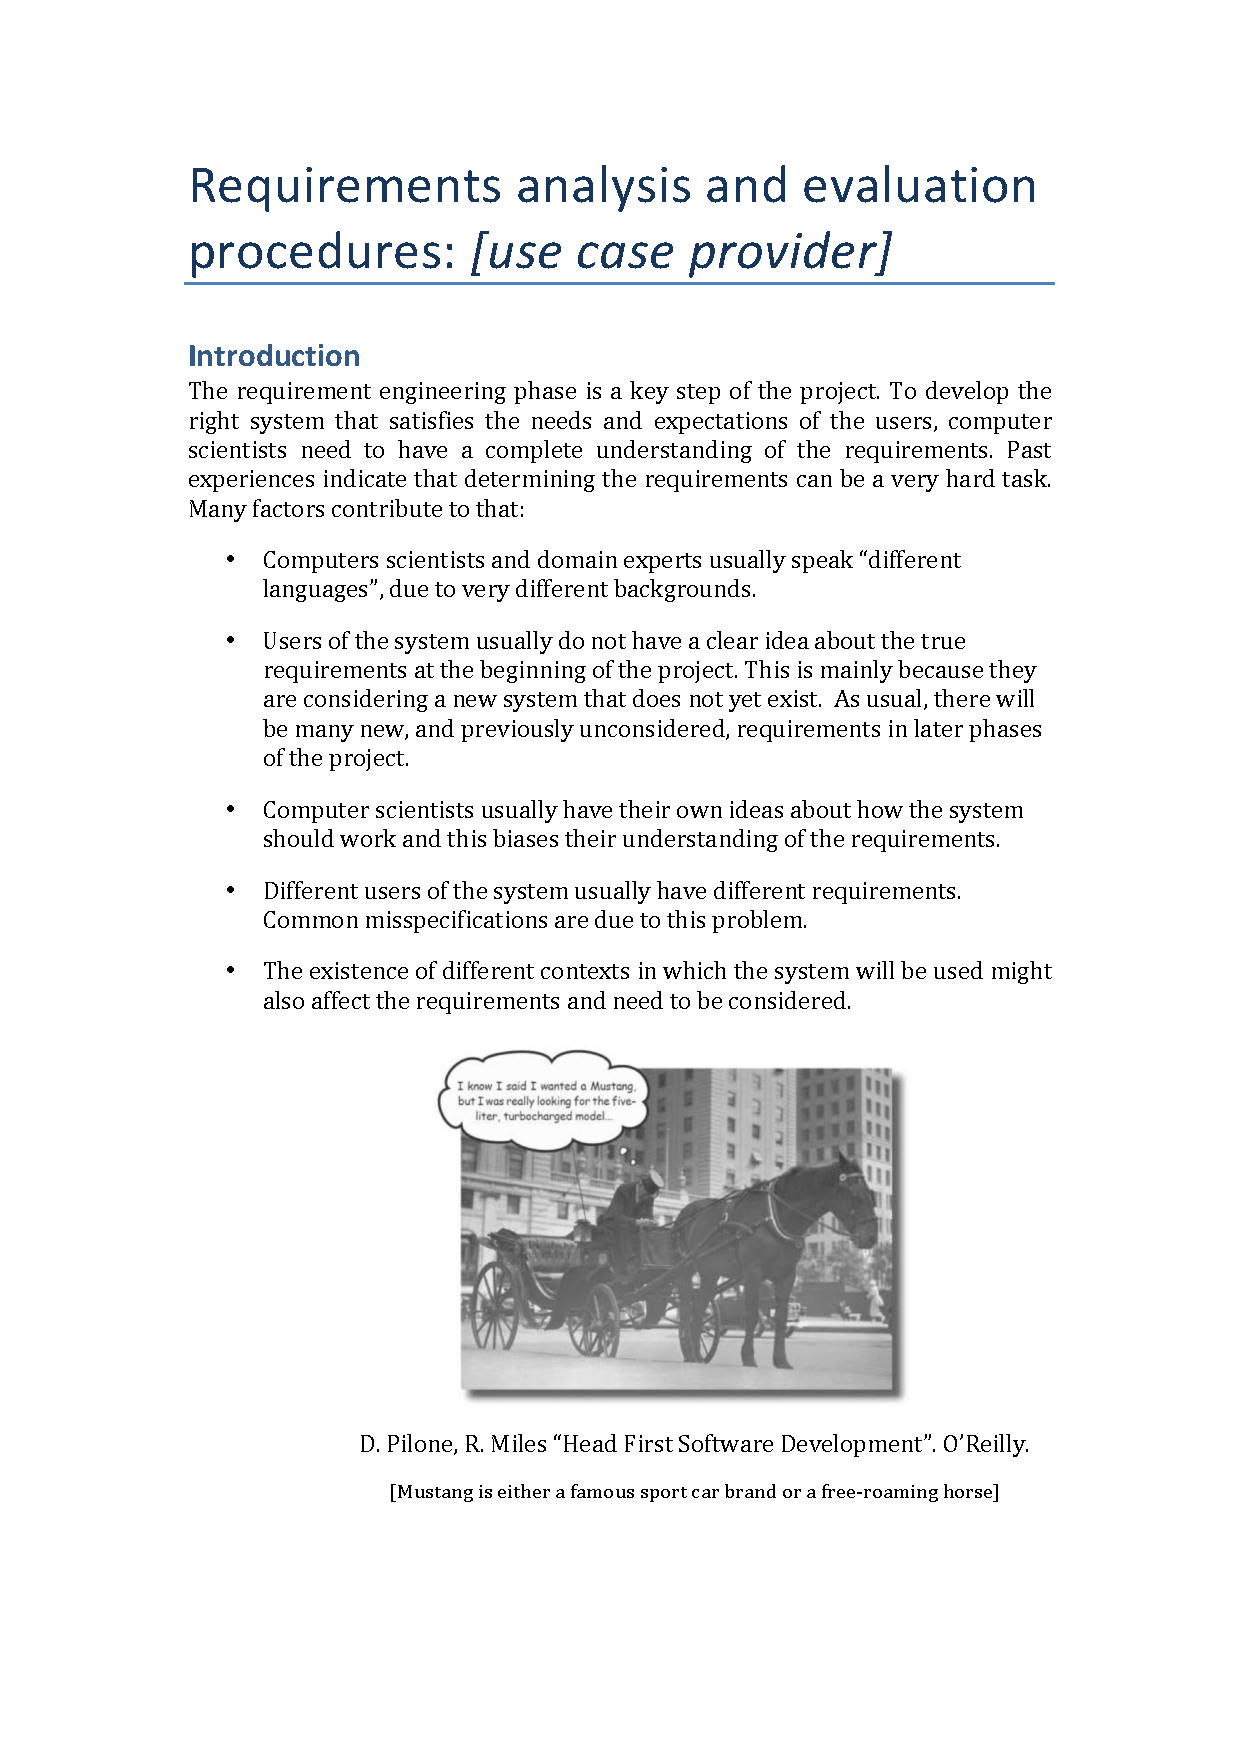
\includepdf[offset=0 1cm,scale=0.85,pages={-},pagecommand={\pagestyle{fancy}}]{appendixA1.pdf}
%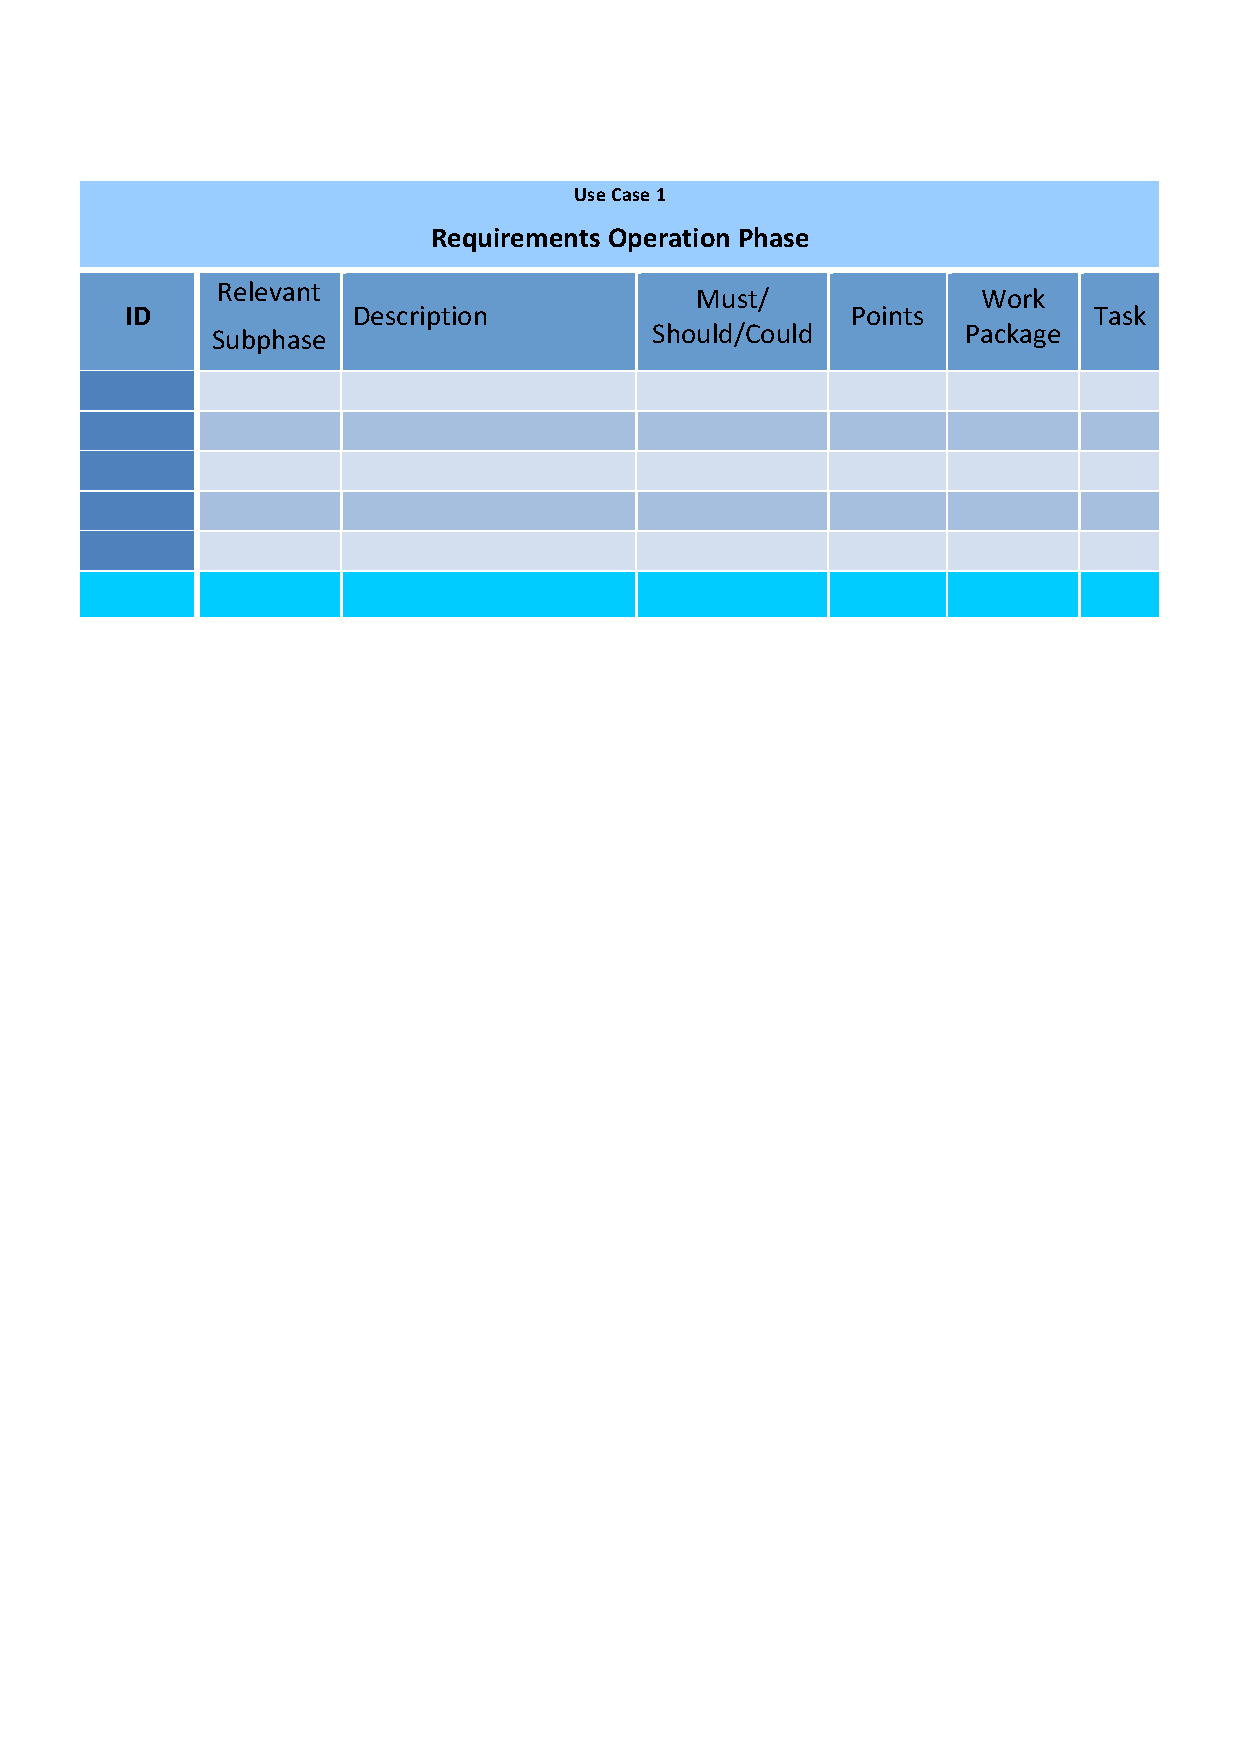
\includepdf[offset=0 1cm,scale=0.85,pages={-},pagecommand={\pagestyle{fancy}}]{appendixA2.pdf}
%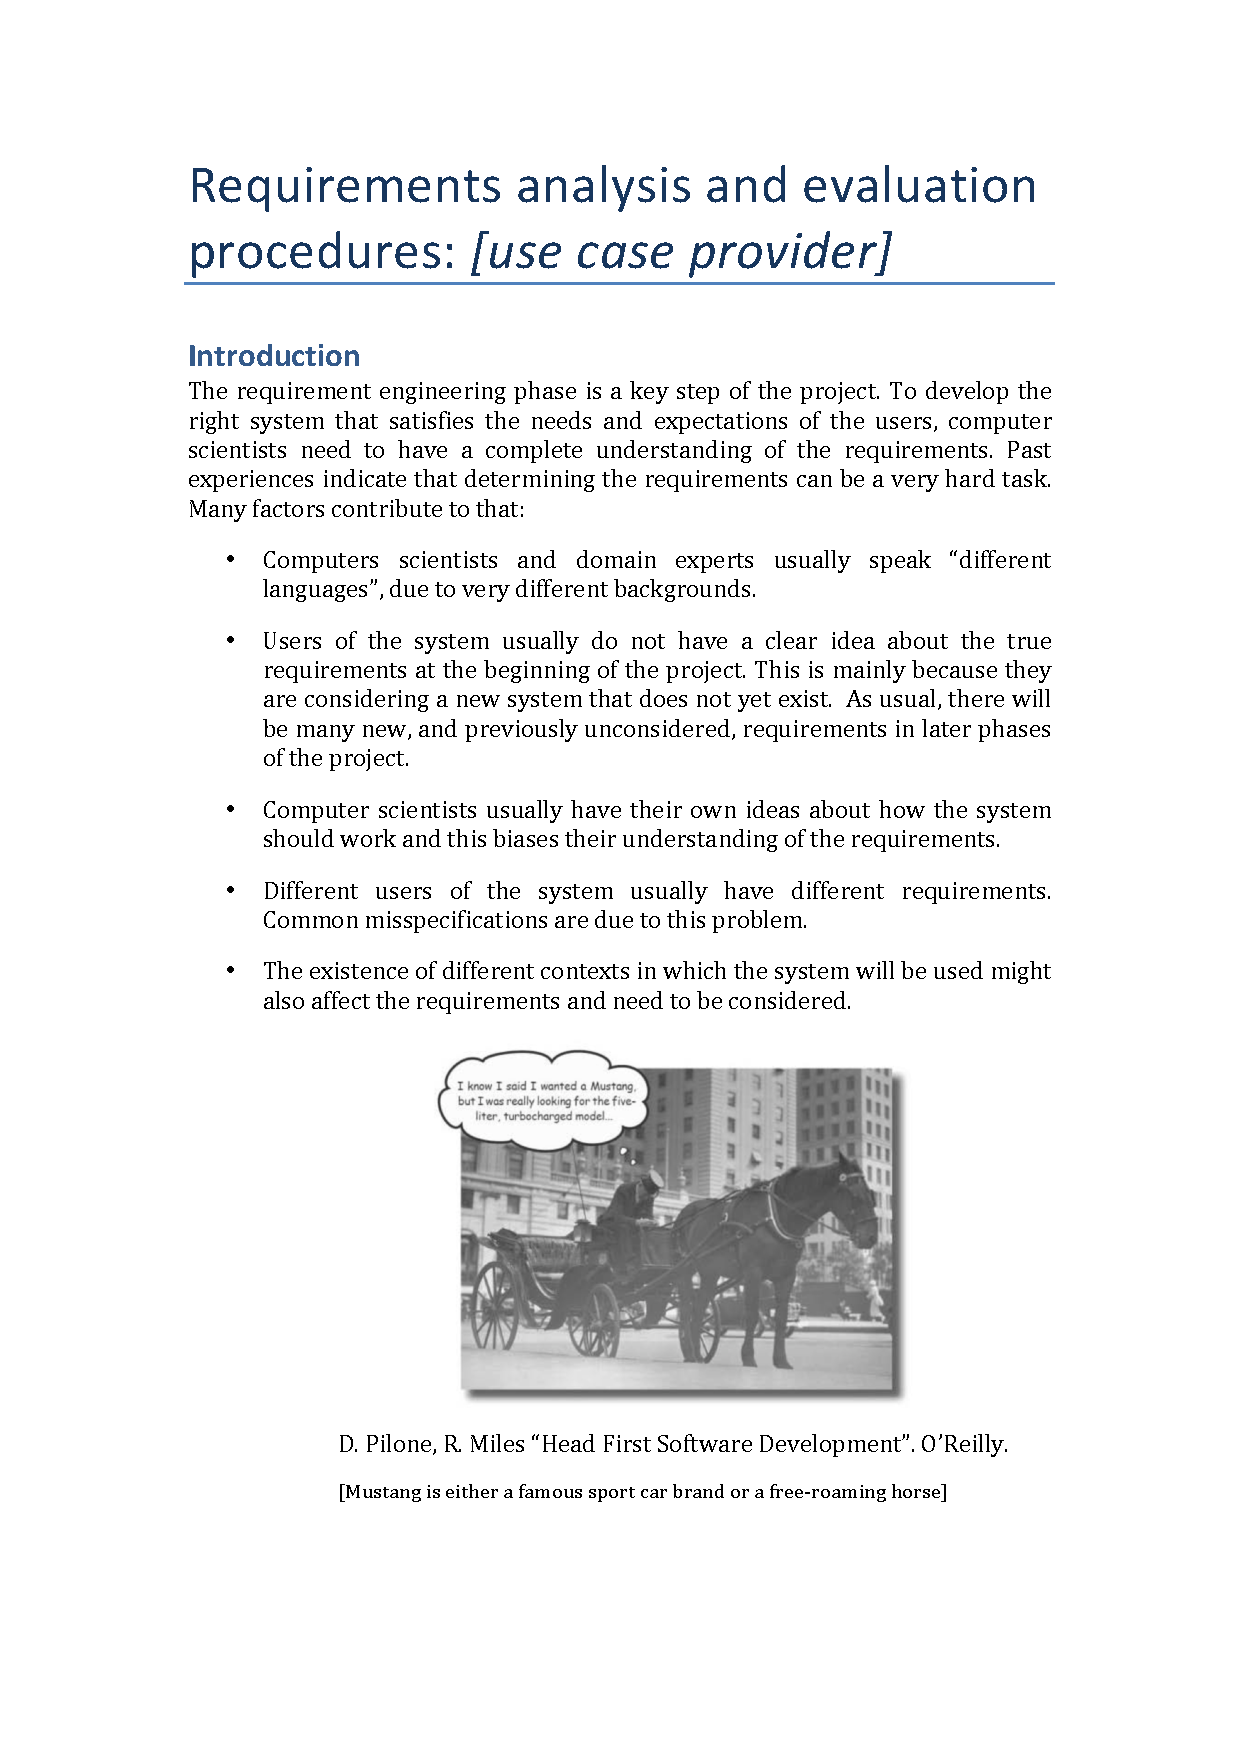
\includepdf[offset=0 1cm,scale=0.85,pages={-},pagecommand={\pagestyle{fancy}}]{appendixA_reformat.pdf}


\end{document}  